%\documentclass{article}
\documentclass[unnumsec,webpdf,contemporary,large,namedate]{oup-authoring-template}
\onecolumn
\usepackage{hyperref}
\usepackage{lmodern}
\usepackage{graphicx}
\usepackage{xr}

\begin{document}
\renewcommand{\figurename}{Fig.~S}
\begin{center}
    {\large Tsbrowse: an interactive browser for Ancestral Recombination Graphs}\\[1ex]
    {\large Supplementary Information}
\end{center}
\section{Supplementary Methods}
%\subsection{Simulation of truth dataset (Fig. \ref{fig:Figure_2})}
\subsection{Simulation of truth dataset (Fig.~2)}
\label{subsec:sweep_simulation}
Ancestral
histories of 300 samples were simulated with the \texttt{SweepGenicSelection}
function in \texttt{msprime (version 1.3.3)}. A combination of models was used:
in the recent past, a selective sweep was simulated with a beneficial allele
situated in the middle of a 5 Mb sequence. The frequency of the allele in the
population was set at 0.0001 at the beginning of the sweep. The allele fixed in
the population at a frequency of 0.9999. The strength of selection was set
using the selection coefficient, \textit{s = 0.25}. A time increment,
\textit{dt = 1e-6} was used to step through the sweep. Mutations were added to
the ARG at a rate of 1e-8 per base pair per generation. A recombination rate of 
1e-8 per base pair per generation was used. For simulating history before the occurrence 
of the sweep, a standard coalescent model (Hudson's algorithm \citep{Hudson1983}) was
used until coalescence was achieved.

\subsection{Inference of SARS-CoV-2 ARGs}
The ARG shown in Fig.~S\ref{fig:Supplementary_Figure_1} was inferred with
\texttt{sc2ts}~\citep{zhan2023towards} using the Viridian
dataset~\citep{hunt2024addressing}. It consists of
2,482,157 samples, 
2,689,054 nodes,
2,689,982 edges
and
1,923,169 mutations.
% Trees   348
% Sequence Length 29904.0
% Time Units  days
% Sample Nodes    2482157
% Total Size  1.5 GiB
% Table   Rows    Size    Has Metadata
% Edges   2689982 82.1 MiB
% Individuals 0   24 Bytes
% Migrations  0   8 Bytes
% Mutations   1923169 202.7 MiB
% Nodes   2689054 1.1 GiB
% Populations 0   8 Bytes
% Provenances 1131    1.7 MiB
% Sites   29803   3.1 MiB
Running \texttt{tsbrowse preprocess} on the input \texttt{tszip} file (113M)
required 2m19s of elapsed time (15m15s CPU time) on an Intel Core(TM) i7-9700 CPU.
The resulting \texttt{.tsbrowse} file size was 130M.
% Preprocessing completed. You can now view with `python -m tsbrowse serve v1-beta1_2023-02-21.pp.md.il.ts.tsbrowse`

% real    2m19.028s
% user    15m15.049s
% sys     0m8.159s
% ```
% Sizes:
% ```
% $ ls -lh v1-beta1_2023-02-21.pp.md.il.ts.ts*
% -rw-rw-r-- 1 jk jk 130M Mar 27 15:08 v1-beta1_2023-02-21.pp.md.il.ts.tsbrowse
% -rw-r--r-- 1 jk jk 113M Mar 27 15:04 v1-beta1_2023-02-21.pp.md.il.ts.tsz
% ```

\subsection{Inference of 1000 Genomes dataset (Fig.~S\ref{fig:Supplementary_Figure_2}, 
Fig.~S\ref{fig:Supplementary_Figure_4})} The 1000 Genomes dataset was downloaded from
\texttt{\url{https://ftp.1000genomes.ebi.ac.uk/vol1/ftp/data_collections/1000G_2504_high_coverage/working/20220422_3202_phased_SNV_INDEL_SV/}}.
The ancestral fasta sequence for chromosome 17 (GRCh38) was downloaded
from the Ensembl database. Inference was performed with a Snakemake pipeline
(\texttt{\url{https://github.com/benjeffery/tsinfer-snakemake/}}) using
\texttt{tsinfer version 0.3.3} for the long arm of chromosome 17 after
filtering out duplicate variant positions, variants with missing or low quality
ancestral allele, singletons, n-1-tons and n-2-tons. Only bi-allelic SNPs were
included for inference. For Supplementary Figure \ref{fig:Supplementary_Figure_4}, 
\texttt{tsdate version 0.2.1} was used to estimate the age of ancestral nodes
 with \textit{mutation rate = 1.29e-8}, setting all other parameters to default 
 values. 

\subsection{Inference of selective sweep dataset (Fig.~S\ref{fig:Supplementary_Figure_3})} 
The following software was used to infer ARGs from the truth dataset described in the
section ``Simulation of truth dataset'' above: 
\texttt{tsinfer version 0.3.3}
\citep{kelleher2019inferring}, \texttt{tsdate version 0.2.1}, 
\texttt{Relate version 1.2.2} \citep{speidel2019method}, 
\texttt{ARG-needle version 1.0.3} \citep{zhang2023biobank},
\texttt{SINGER version 0.1.8-beta} \citep{deng2024robust}.
For all inferences, the following parameters were used: \textit{recombination
    rate = 1e-8}, \textit{mutation rate = 1e-8}, \textit{effective population size
    = 10,000}. Default values were used for other parameters.

\subsection{Code availability} Code to recreate datasets used in this paper are available at:
\texttt{\url{https://github.com/savitakartik/tsbrowse-paper}}.

\clearpage
\section{Supplementary Figures}
\begin{figure}[h]
    \centering
    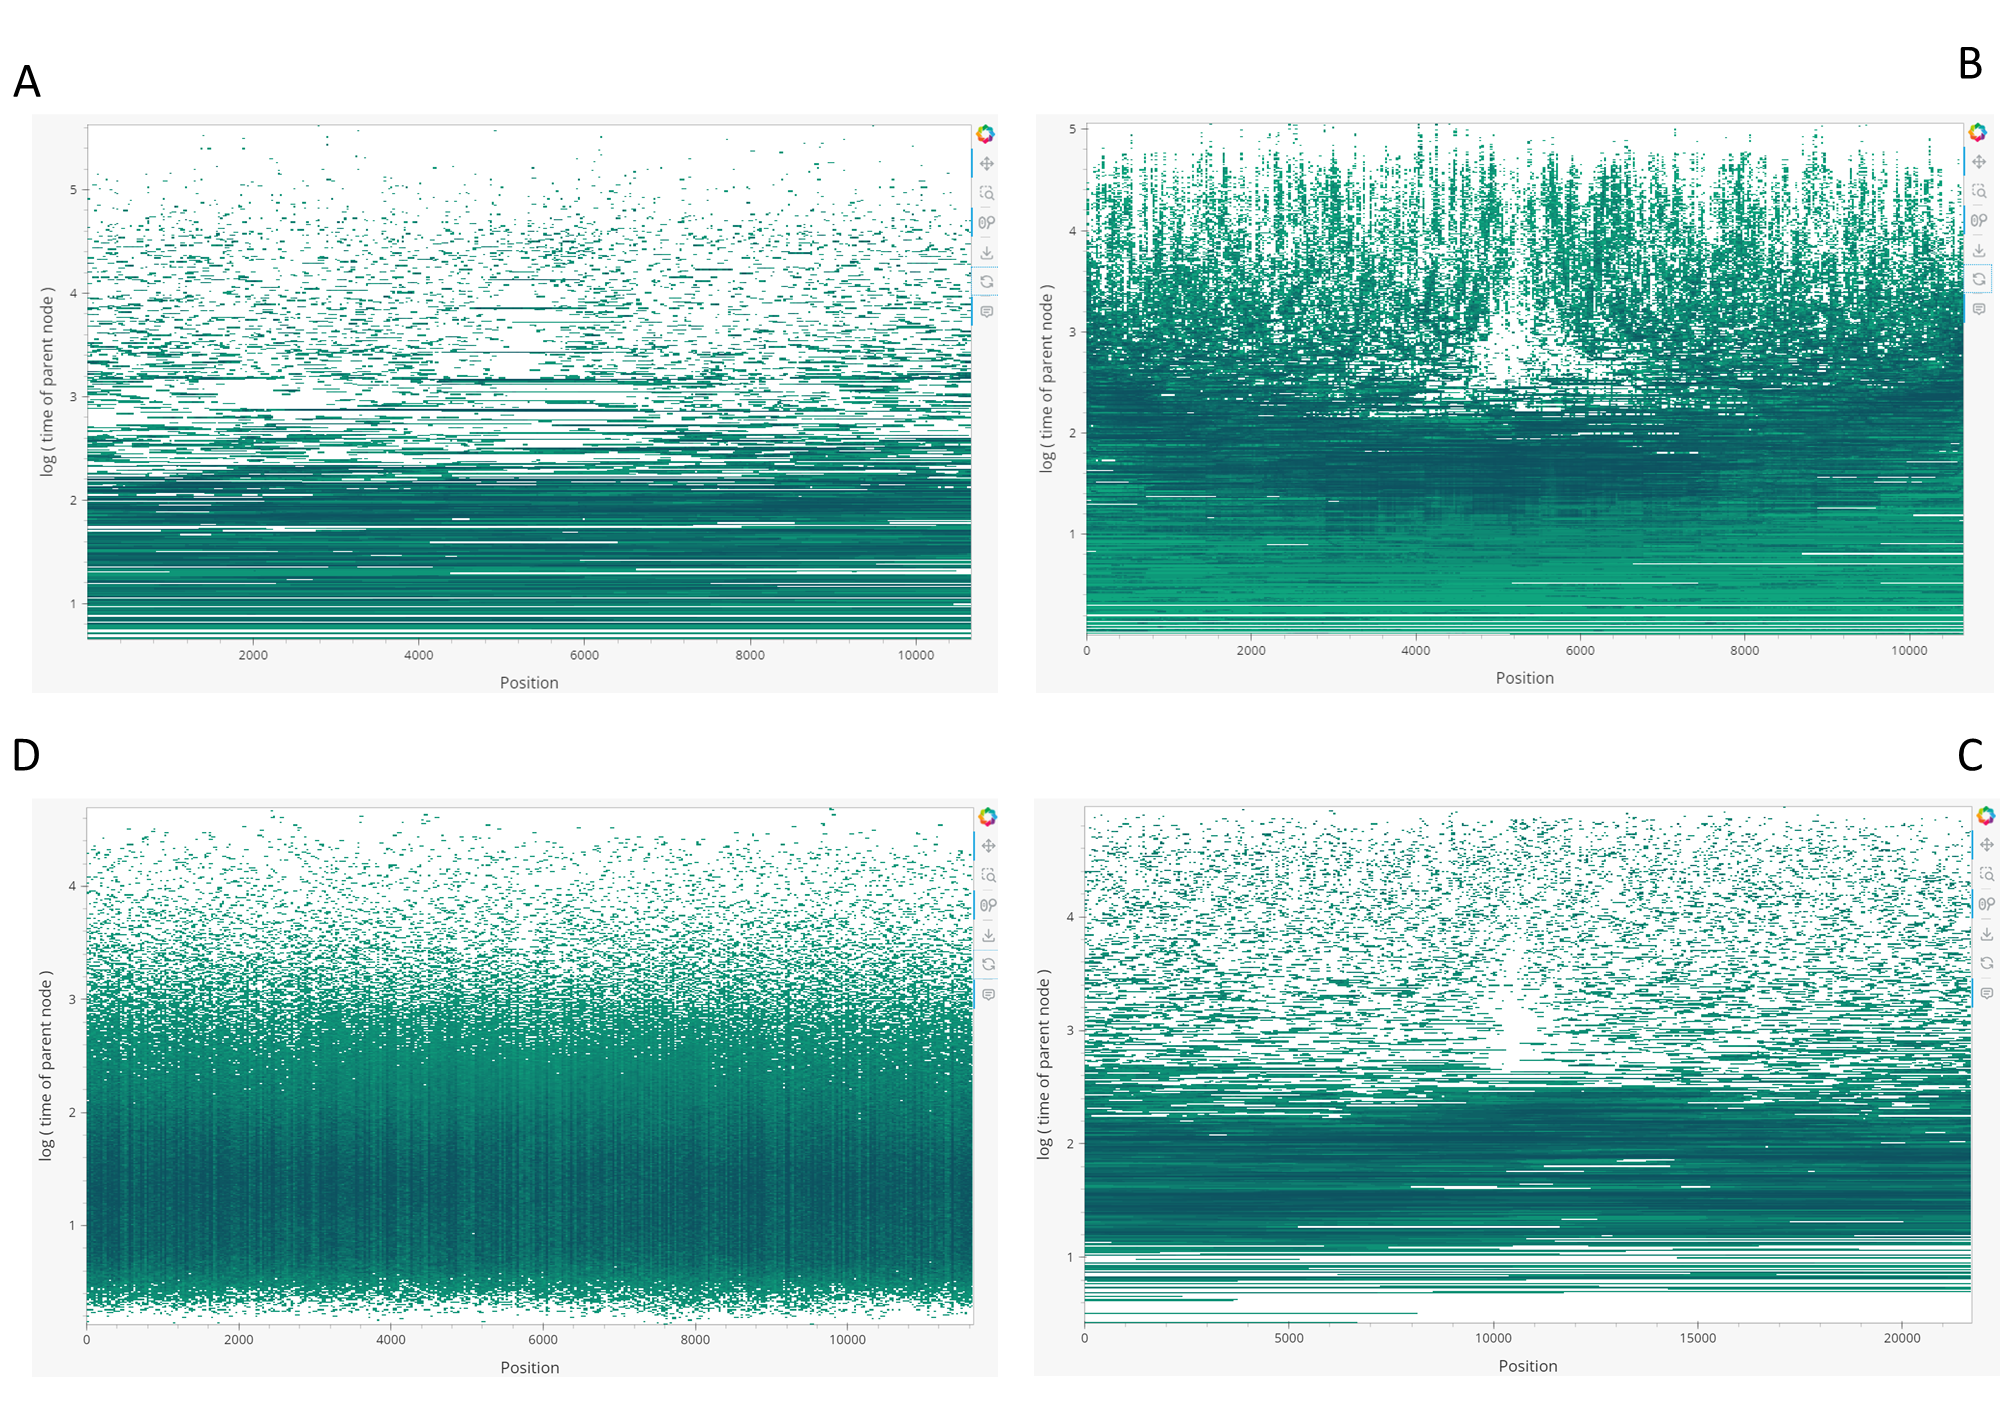
\includegraphics[width=0.95\linewidth]{figures/SuppFig1.png}
    \caption{\textbf{\texttt{tsbrowse} applied to SARS-CoV-2 ARGs.}
        A screenshot of \texttt{tsbrowse}'s depiction of
        1,923,169 mutations in an
        ARG inferred by \texttt{sc2ts}; see text for details. Also shown are the
        gene annotations along the X-axis.}
    \label{fig:Supplementary_Figure_1}
\end{figure}

\begin{figure}
    \centering
    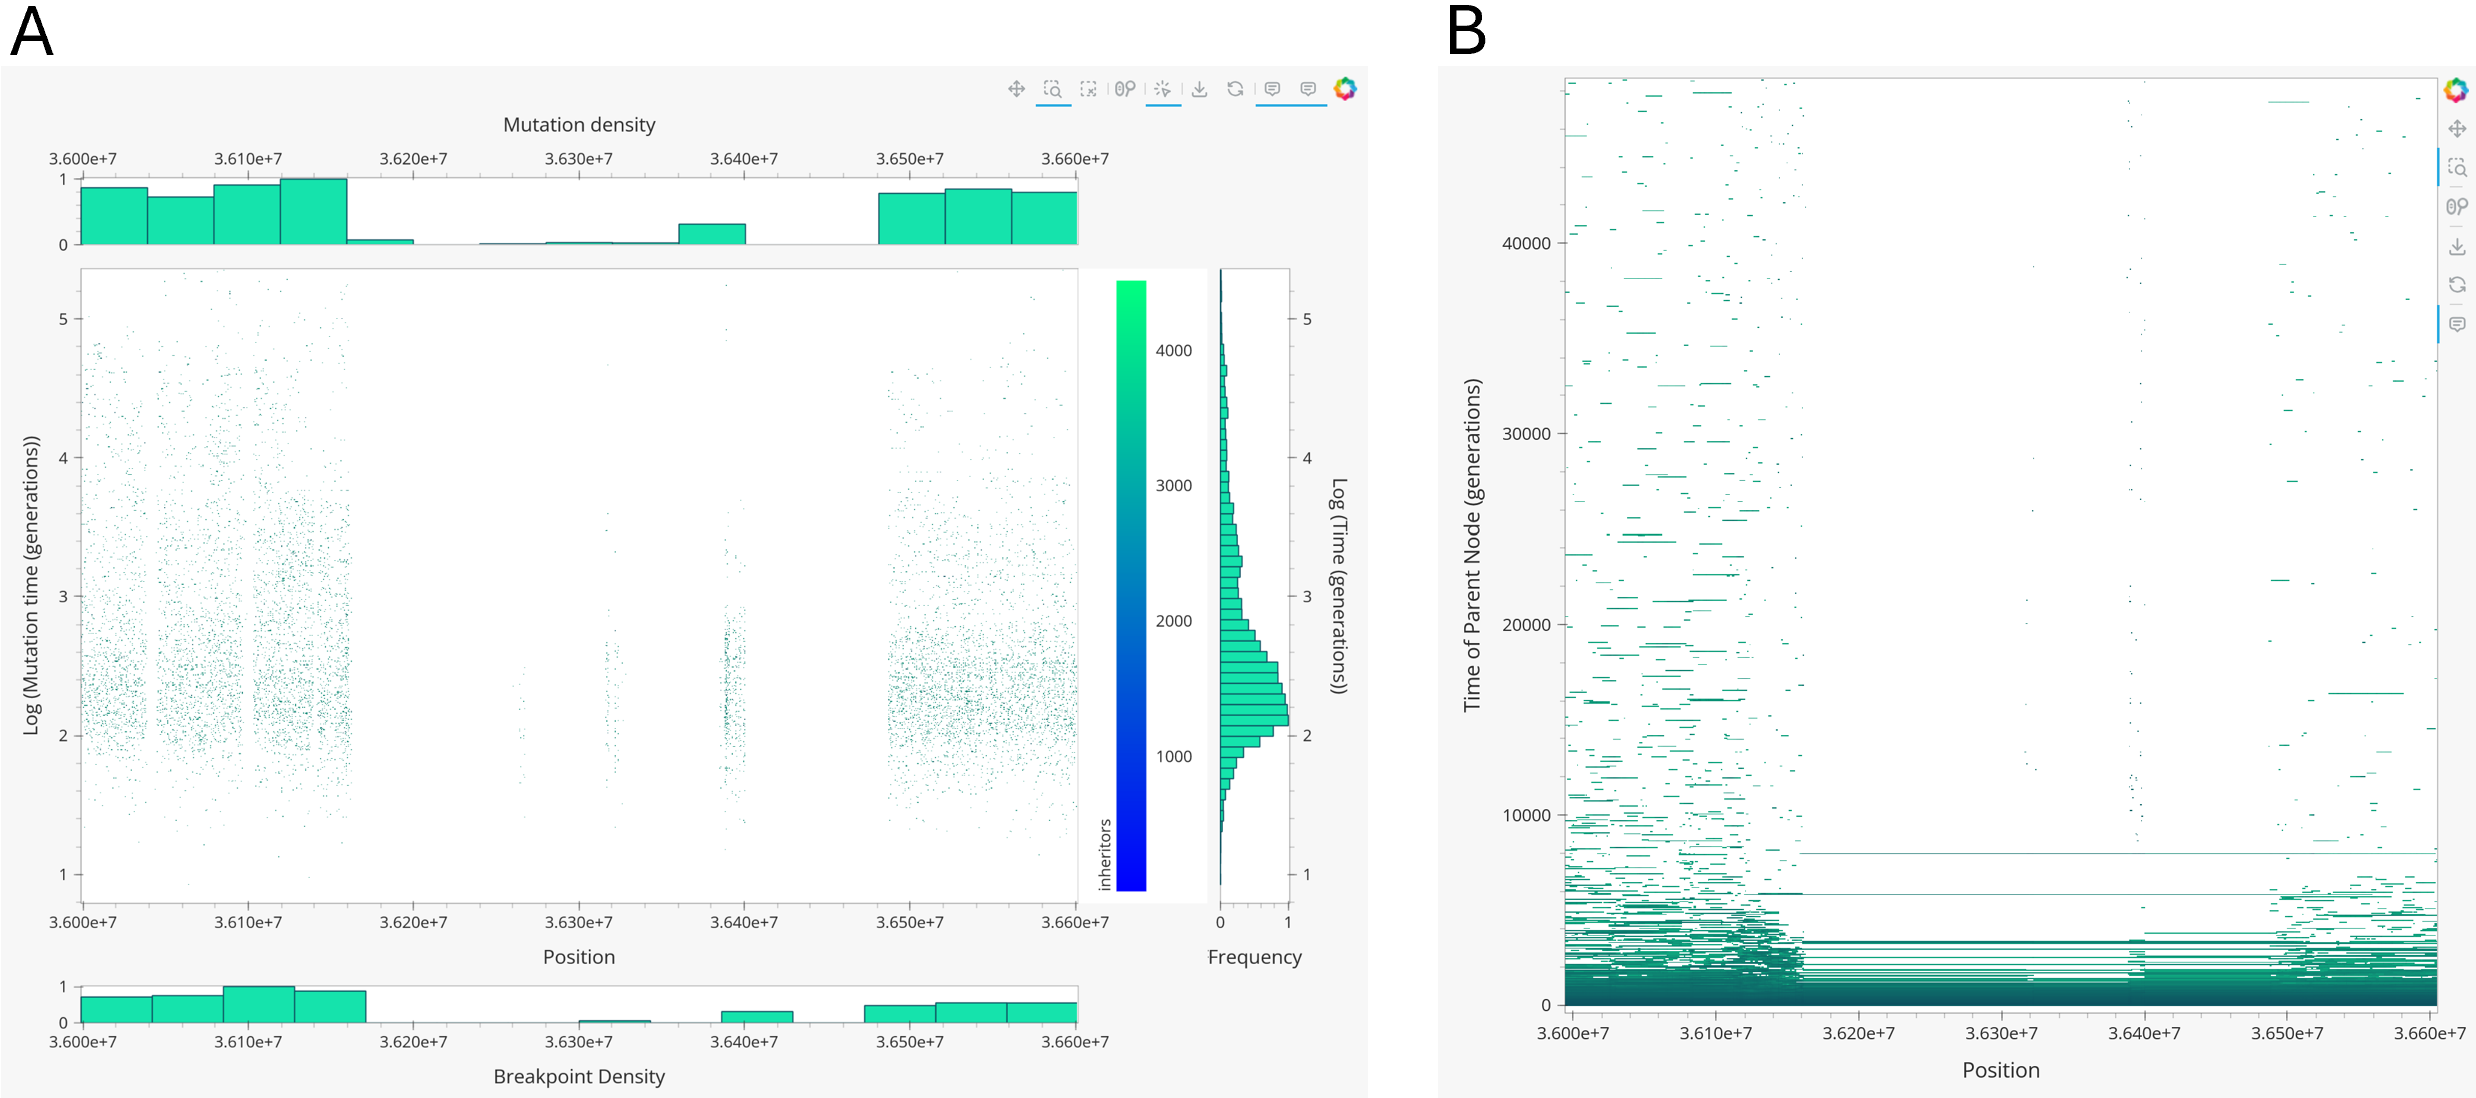
\includegraphics[width=0.95\linewidth]{figures/SuppFig2.png}
    \caption{\textbf{Nodes view for a 1000 Genomes inference.} A
        screenshot of \texttt{tsbrowse}'s Nodes view for an inference of the long arm
        of chromosome 17 from the 1000 Genomes whole-genome sequencing dataset. At the
        top is a plot of node spans over time. The length of sequence that the nodes
        span is shown on the X axis, and the time of nodes is shown on the Y axis. The
        histogram at the bottom shows the distribution of node spans. }
    \label{fig:Supplementary_Figure_2}
\end{figure}

\begin{figure}
    \centering
    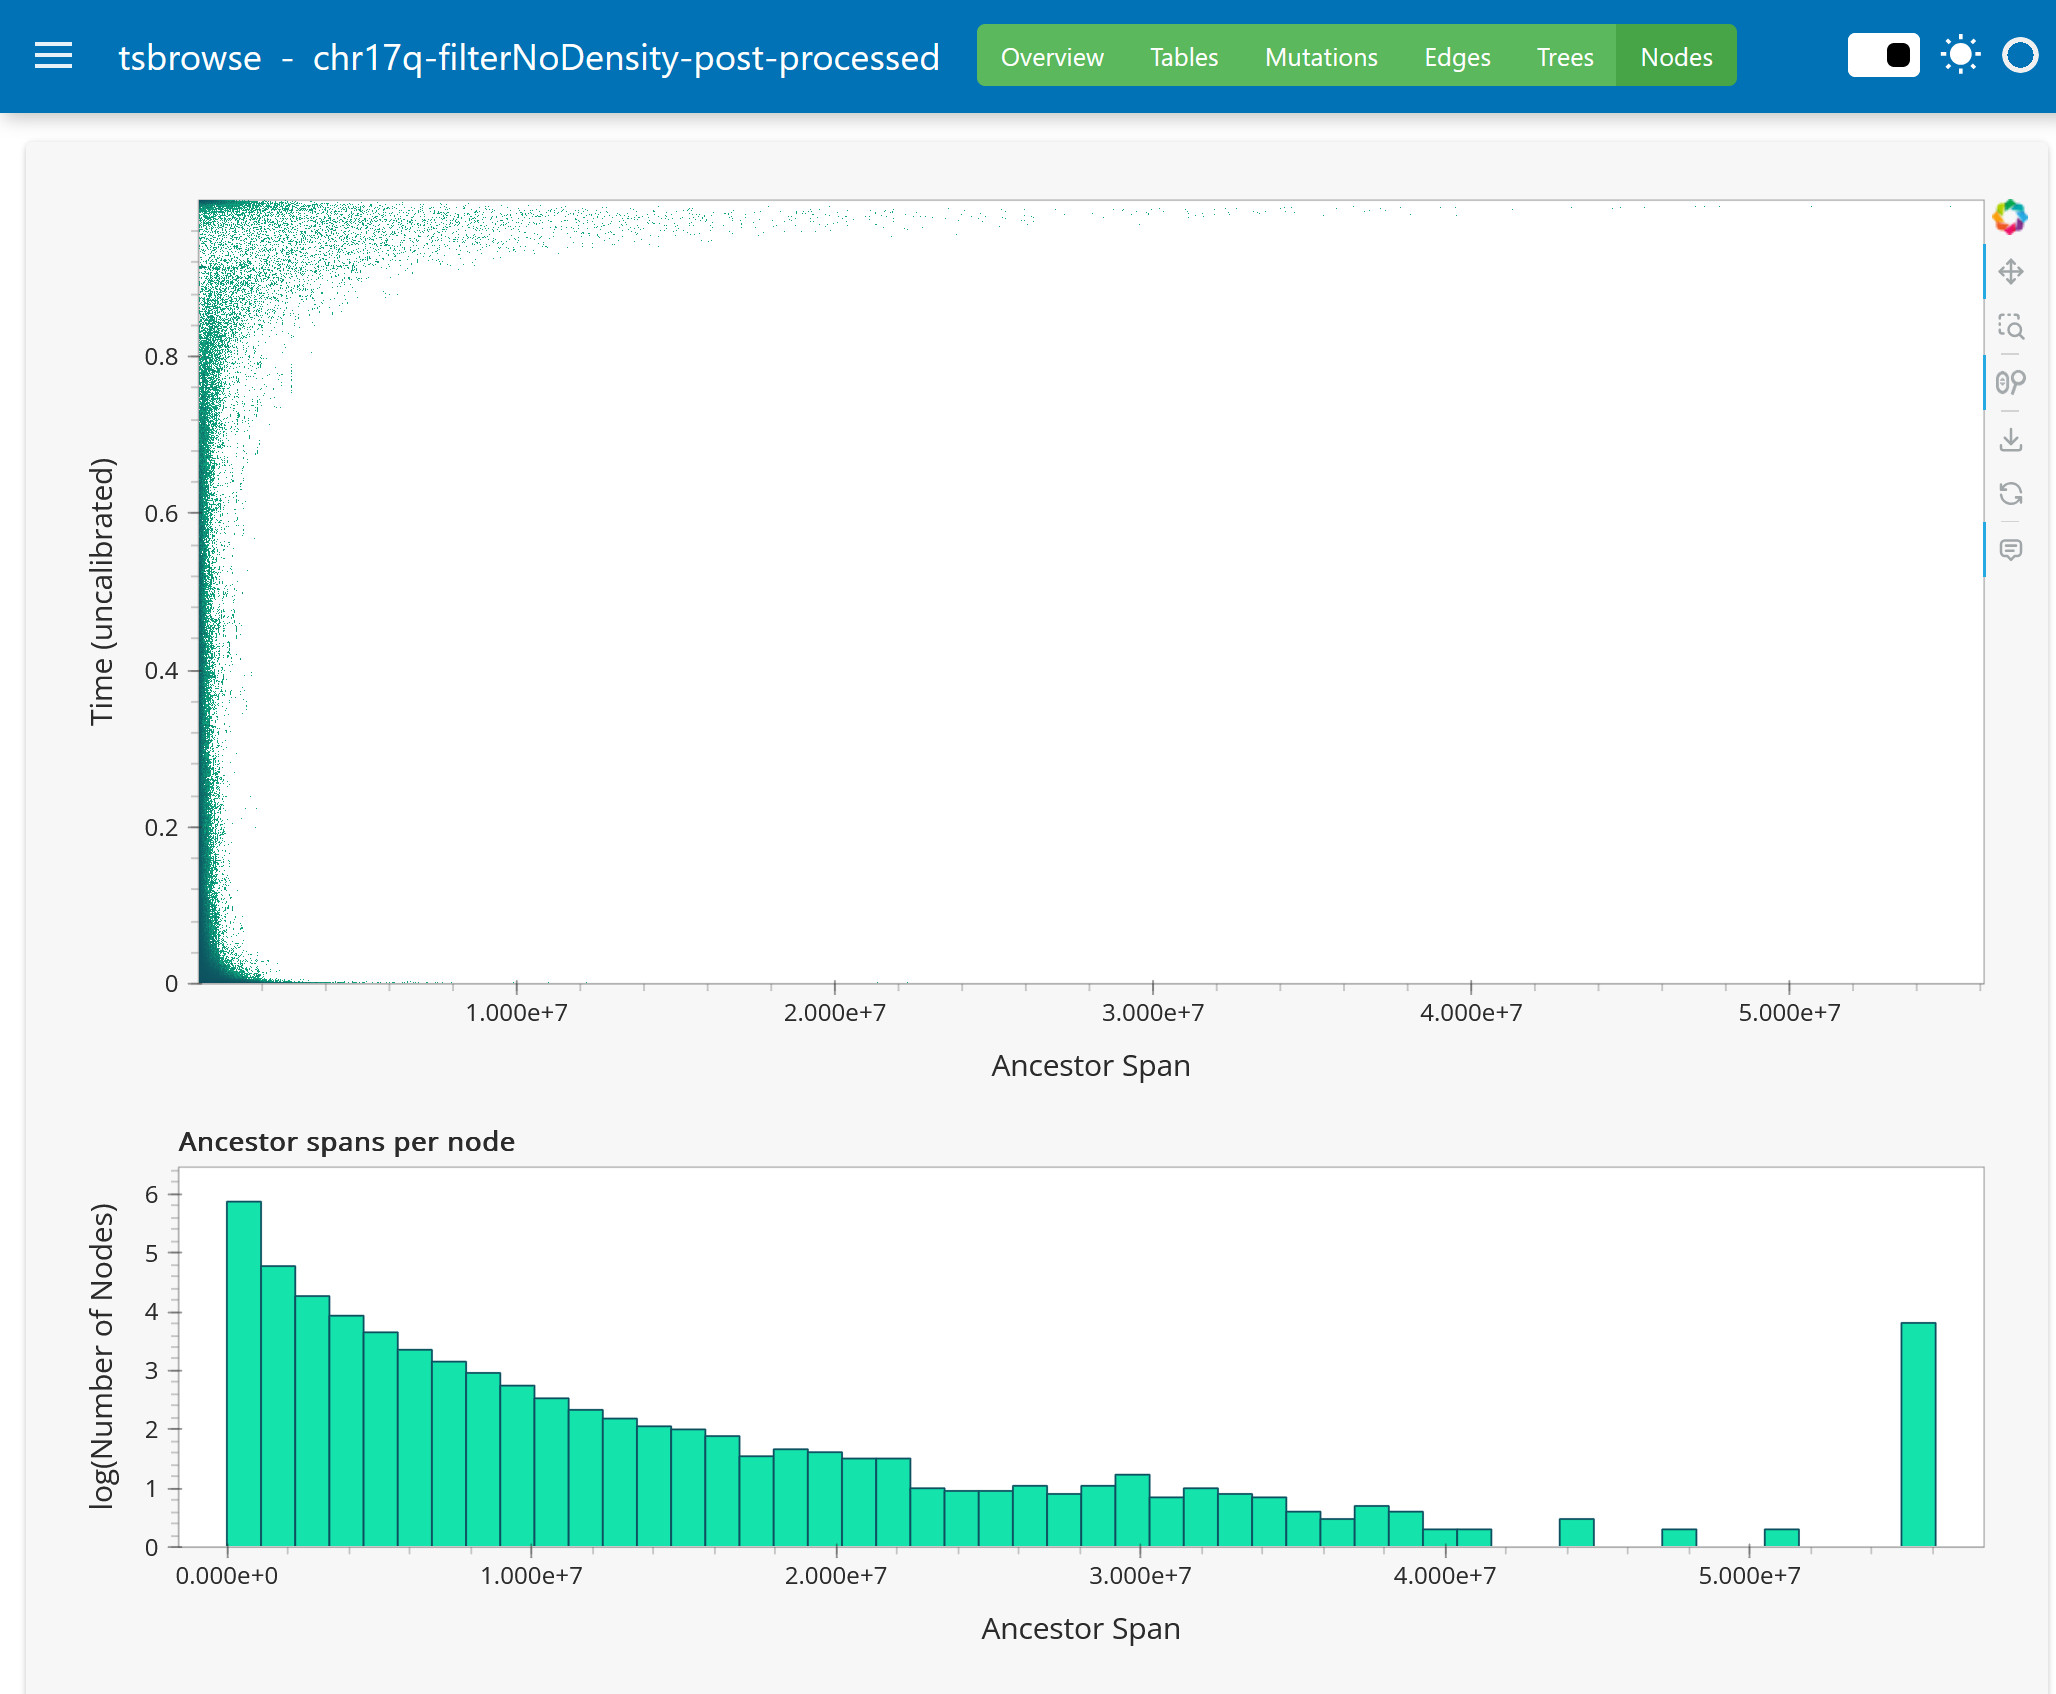
\includegraphics[width=0.95\linewidth]{figures/SuppFig3.png}
    \caption{\textbf{\texttt{Tsbrowse} applied to inference methods.}
    A screenshot of \texttt{tsbrowse}'s Edges view for tsinfer+tsdate,
ARG-Needle, Relate and SINGER inferences of the truth dataset
simulated under a selective sweep model (shown in Figure 2 of the main text). For
SINGER, one of the posterior ARG samples is shown.
The X coordinate represents genomic position, each horizontal segment on the
plot shows the genomic coordinates that the edge spans, and Y coordinate shows
time of either the parent or child node in the edge.}
    \label{fig:Supplementary_Figure_3}
\end{figure}

\begin{figure}
    \centering
    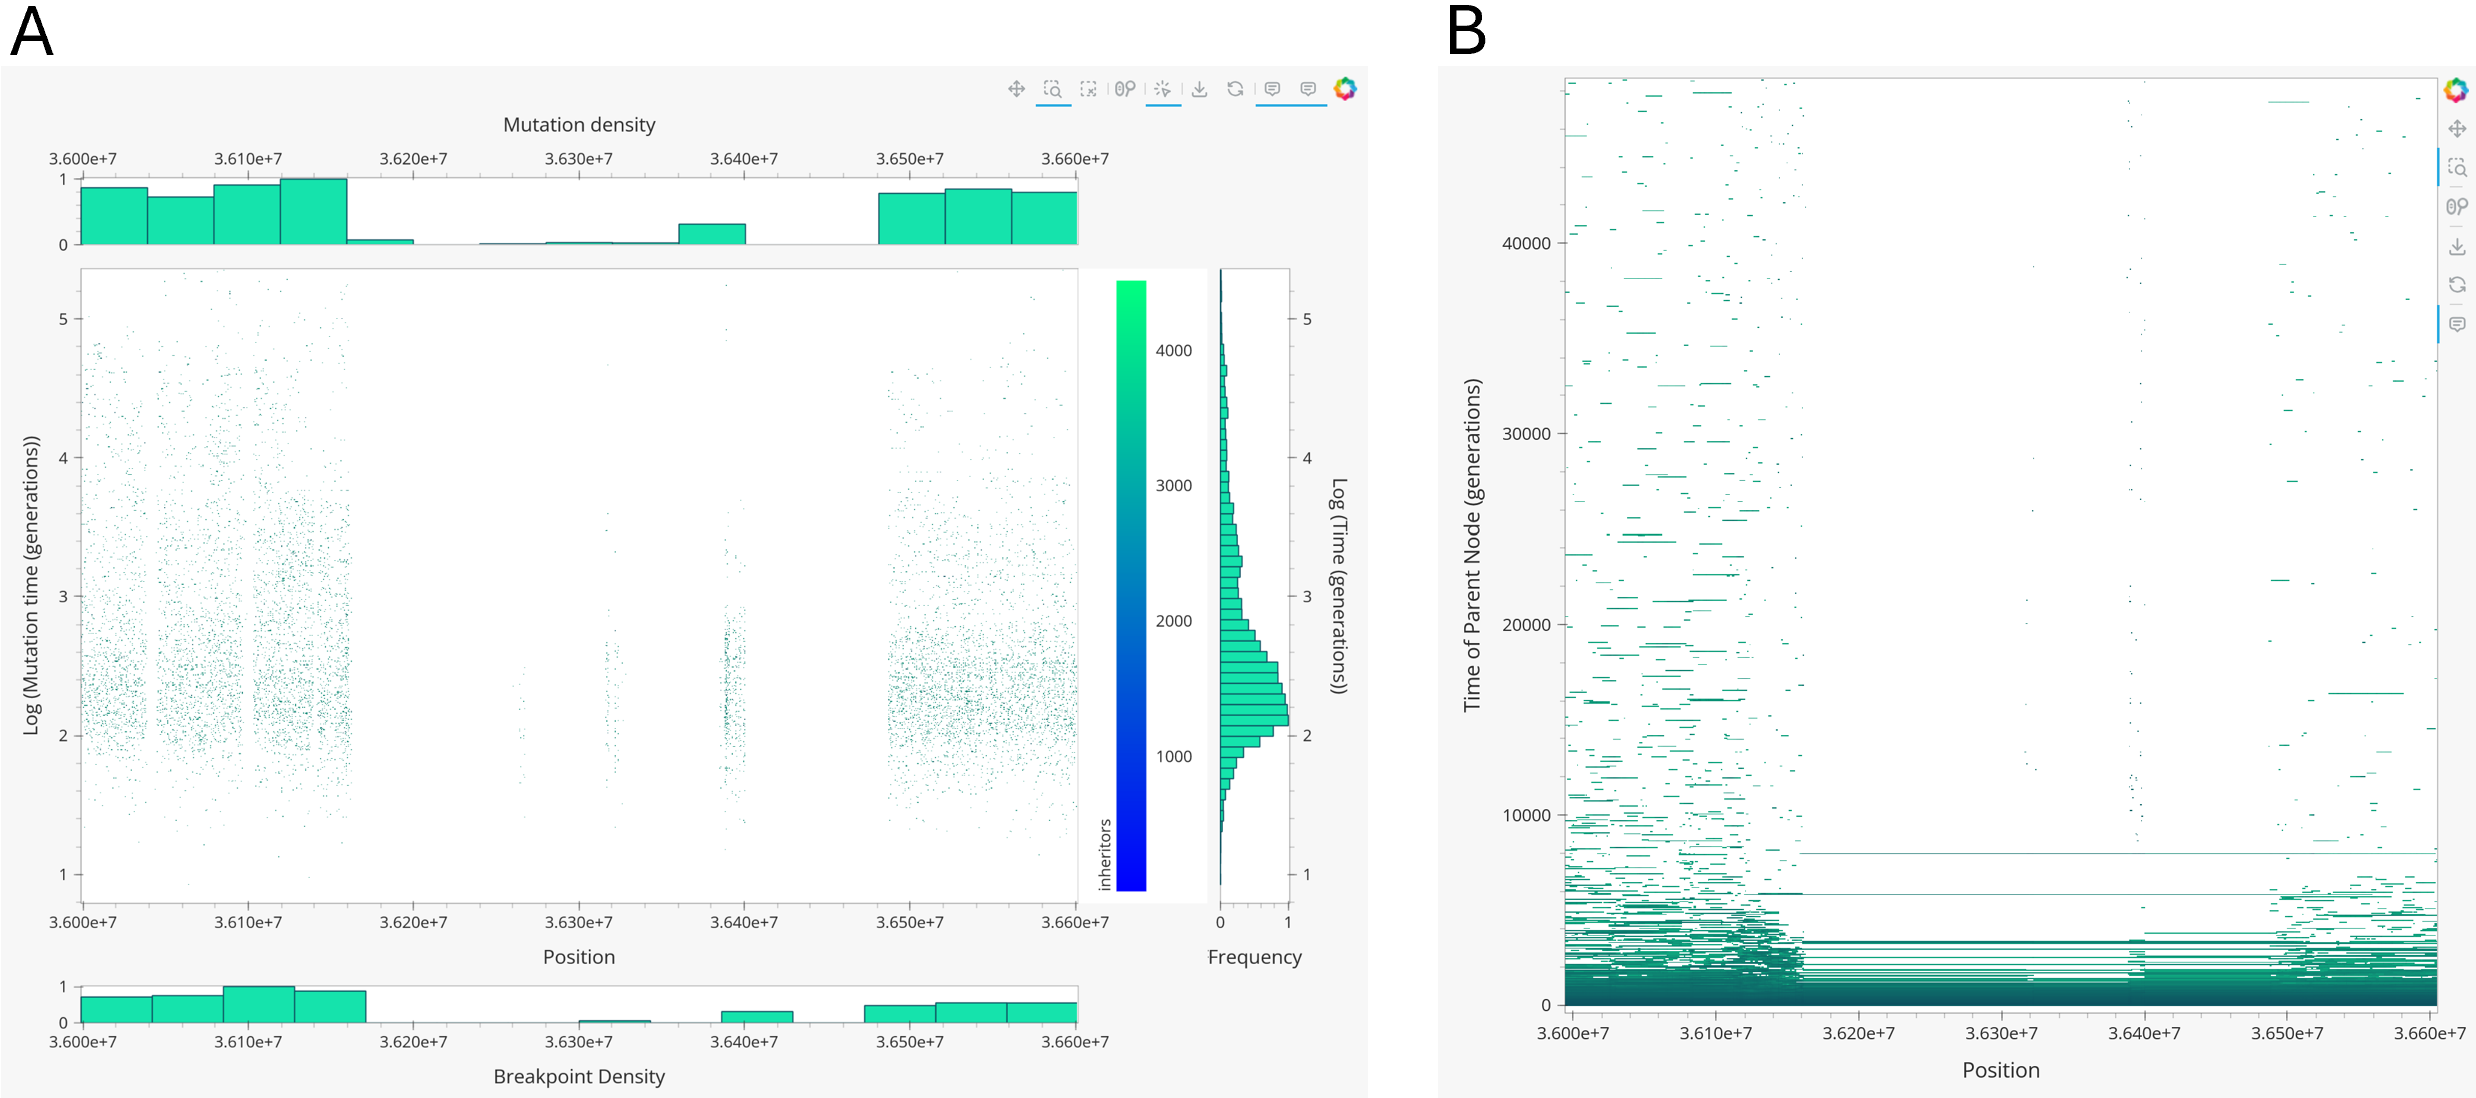
\includegraphics[width=0.95\linewidth]{figures/SuppFig4.png}
    \caption{\textbf{Identifying ARG inference problems with \texttt{tsbrowse}.} 
Screenshots of \texttt{tsbrowse}'s Mutations view (A) and Edges view (B) for a
 600 kb region of chromosome 17 inferred from 3,202 participants from the 1000 
 Genomes Whole Genome Sequencing dataset \citep{1000GWGS}. 
 The poor performance of \texttt{tsinfer} in this variant-poor region is evidenced
  by the long edges spanning gaps in mutation density.}
    \label{fig:Supplementary_Figure_4}
\end{figure}
\clearpage
\bibliographystyle{natbib}
\bibliography{reference}
\end{document}
